\paragraph{}
La idea de esta sección es proponer algunos tipos de expansiones en serie y ver como se podrían implementar utilizando bancos de filtros.

\subsection{Expansión De Haar}

\paragraph{}
La primera de las expansiones será la de Haar, dicha expansión es ortonormal y se basa en la siguiente base de funciones:

\[ \phi_{2k}[n] = \begin{cases} 
      \frac{1}{\sqrt{2}} & n = 2 k, 2 k + 1 \\
      0 & otro \, caso
   \end{cases}
\]

\[ \phi_{2k + 1}[n] = \begin{cases} 
      \frac{1}{\sqrt{2}} & n = 2 k \\
      -\frac{1}{\sqrt{2}} & n = 2 k + 1 \\
      0 & otro \, caso
   \end{cases}
\]

\paragraph{}
La idea sería demostrar que esta expansión puede implementarse con una estructura de bancos de filtros. La estructura a utilizar es la de la figura \ref{fig:banco_de_2}.

	\begin{figure}[h!]
		\centering
		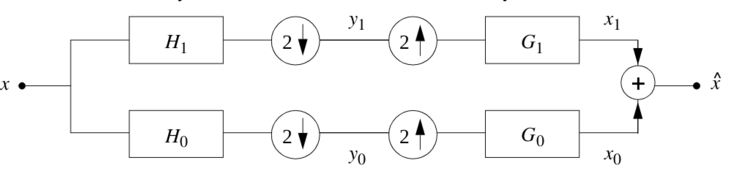
\includegraphics[width=1.0\textwidth, trim = 0cm 0cm 0cm 0cm]{banco_de_2.png}
		\caption{Banco de filtros de dos canales.}
		\label{fig:banco_de_2}
	\end{figure}
	
\paragraph{}
Dicha estructura se compone de una parte de analisis, compuesta por los filtros $H_{0}$ y $H_{1}$, junto con los dos Downsamplers de 2. El objetivo de la parte de analisis es poder computar en las salidas $y_{0}$ e $y_{1}$ los coeficientes de la expansion. La parte de sintesis esta compuesta por los filtros $G_{0}$ y $G_{1}$, junto con los Upsamplers de 2. El objetivo de la parte de sintesis es poder recuperar la señal original a la salida. Si la reconstrucción es perfecta, la salida será una versión posiblemente retrasada de la señal de entrada.

\paragraph{}
Lo primero que se debe ver es que los coeficientes de la expansión se pueden calcular de la siguiente manera:

\begin{equation}
	X[2k] = \langle \phi_{2k} , x \rangle = \frac{1}{\sqrt{2}} (x[2k] + x[2k + 1])
\end{equation}

\begin{equation}
	X[2k + 1] = \langle \phi_{2k + 1} , x \rangle = \frac{1}{\sqrt{2}} (x[2k] - x[2k + 1])
\end{equation}

\paragraph{}
Es decir que los coeficientes pares son el promedio de dos muestras seguidas, y los impares la primera diferencia entre dos muestras seguidas. El siguiente paso es poder elegir los filtros $H$. Si se elige los filtros de la siguiente manera:

\[ h_{0}[n] = \begin{cases} 
      \frac{1}{\sqrt{2}} & n = -1, 0 \\
      0 & otro \, caso
   \end{cases}
\]

\[ h_{1}[n] = \begin{cases} 
      \frac{1}{\sqrt{2}} & n = -1 \\
      -\frac{1}{\sqrt{2}} & n = 0 \\
      0 & otro \, caso
   \end{cases}
\]

\paragraph{}
Los coeficientes se pueden obtener de la siguiente manera:

\begin{equation}
  \left.h_{0}[n] * x[n]\right\vert_{n = 2k} = \sum_{l \in \mathbb{Z}} h_{0}[2k - l] x[l] = \frac{1}{\sqrt{2}} (x[2k] + x[2k + 1]) = X[2k]
\end{equation}

\begin{equation}
  \left.h_{1}[n] * x[n]\right\vert_{n = 2k} = \sum_{l \in \mathbb{Z}} h_{1}[2k - l] x[l] = \frac{1}{\sqrt{2}} (x[2k] - x[2k + 1]) = X[2k + 1]
\end{equation}

\paragraph{}
Observar que evaluar el resultado de la salida del filtro en $2k$ es equivalente a hacer un Downsampling en 2. De esta forma hemos podido computar los coeficientes de la transformación en las salidas $y_{0}$ e $y_{1}$:

\begin{equation}
  y_{0}[k] = X[2k]
\end{equation}

\begin{equation}
  y_{1}[k] = X[2k + 1]
\end{equation}

\paragraph{}
Observar también que las respuestas impulsivas de los filtros son versiones invertidas en el tiempo de las señales de la base:

\begin{equation}
  h_{0}[n] = \phi_{0}[-n]
\end{equation}

\begin{equation}
  h_{1}[n] = \phi_{1}[-n]
\end{equation}

\paragraph{}
En cuanto a la parte de reconstrucción, debemos elegir los filtros $g_{0}$ y $g_{1}$ de forma que la reconstrucción sea perfecta. Se elegirá los filtros de la siguiente manera:

\begin{equation}
  g_{0}[n] = \phi_{0}[n]
\end{equation}

\begin{equation}
  g_{1}[n] = \phi_{1}[n]
\end{equation}

\paragraph{}
Observando que:

\begin{equation}
  \phi_{2k}[n] = g_{0}[n - 2k]
\end{equation}

\begin{equation}
  \phi_{2k + 1}[n] = g_{1}[n - 2k]
\end{equation}

\paragraph{}
Se puede ver que se recupera la señal $x[n]$:

\begin{equation}
  x[n] = \sum_{k \in \mathbb{Z}} X[k] \phi_{k}[n] = \sum_{k \in \mathbb{Z}} y_{0}[k] \phi_{2k}[n] + \sum_{k \in \mathbb{Z}} y_{1}[k] \phi_{2k + 1}[n] = \sum_{k \in \mathbb{Z}} y_{0}[k] g_{0}[n - 2k] + \sum_{k \in \mathbb{Z}} y_{1}[k] g_{1}[n - 2k]
\end{equation}

\paragraph{}
Ver que cada muestra de $y_{i}[k]$ suma una copia de la respuesta impulsiva de $g_{i}[n]$ desplazada en $2k$. Esto puede ser implementado mediante un Upsampling en 2 (Insertando un 0 entre cada dos muestras de $y_{i}[k]$). De esta forma hemos realizado la reconstrucción de la señal utilizando la parte de sintesis del banco de filtros. Con esta elección de los filtros, nuestro banco de filtros de la figura \ref{fig:banco_de_2} es un banco de filtros de reconstrucción perfecta, de dos canales, que implementa la expansión en series de Haar.

\subsection{Expansión Sinc}

El objetivo de la presente sección era poder demostrar la conexión que hay entre los bancos de filtros y las expansiones en serie, incluyendo alguna idea intuitiva de lo que significa reconstrucción perfecta. Si bien este objetivo queda cumplido con la sección anterior, que habla sobre la expansión de Haar, queremos introducir brevemenete la expansión sinc por una cuestión de completitud. La expansión sinc posee cierta dualidad con la expansión de Haar en cierto sentido a exponer. Las funciones base en la expansión de Haar están bien localizadas en el tiempo, ya que se componen de solo dos muestras adyacentes, pero tienen una mala resolución en frecuencia. Las funciones base de la expansión sinc, por el contrario, constituyen las respuestas al impulso de filtros pasabajo y pasaalto ideales. Si bien tienen una resolusión en frecuencia perfecta, tienen una mala localización en el tiempo ya que las respuestas decaen con una proporción de 1/n.

\paragraph{}
Para empezar elegiremos a nuestro $G_{0}$ como un filtro pasabajos ideal:

\[ G_{0}(e^{j\omega}) = \begin{cases} 
      \sqrt{2} & \omega \in [-\frac{\pi}{2}, \frac{\pi}{2}] \\
      0 & \omega \in [\frac{\pi}{2}, \frac{3\pi}{2}]
   \end{cases}
\]

\paragraph{}
Que en el tiempo es:

\begin{equation}
  g_{0}[n] = \frac{1}{\sqrt{2}} \frac{sin \pi n / 2}{\pi n / 2}
\end{equation}

\paragraph{}
Para $G_{1}$ se debe elegir un filtro pasaaltos complementario. Para esto, elegimos una versión modulada de $g_{0}[n]$, invertida en el tiempo, con un desplazamiento en 1 (Por una cuestion de completitud de las funciones base):

\begin{equation}
  g_{1}[n] = (-1)^n g_{0}[-n + 1]
\end{equation}

\paragraph{}
En cuanto a los filtros de analisis $h_{i}[n]$, como en el caso anterior, elegimos una version invertida en el tiempo de los filtros de sintesis $g_{i}[n]$:

\begin{equation}
  h_{i}[n] = g_{i}[-n]
\end{equation}

\paragraph{}
De esta forma hemos construido un banco de filtros que implementa la expansion sinc. La expansion sinc, al igual que la Haar, posee funciones base que son versiones con corrimientos pares de los filtros $g_{i}[n]$:

\begin{equation}
  \phi_{2k}[n] = g_{0}[n - 2k]
\end{equation}

\begin{equation}
  \phi_{2k + 1}[n] = g_{1}[n - 2k]
\end{equation}
